\section{Motivating toy example} \label{sec:motivating-example}

%
%
We provide here a toy scenario that illustrates intuitively the pitfalls that may arise when assessing twins using observational data without properly accounting for causal considerations (including unmeasured confounding in particular).
%
Suppose a digital twin has been designed for a particular make of car, e.g.\ to facilitate autonomous driving \citep{allamaa2022sim2real}.
The twin simulates how quantities such as the velocity and fuel consumption of the car respond as certain inputs are applied to it, such as braking, acceleration, steering, etc.
We wish to assess the accuracy of this twin using a dataset obtained from a fleet of the same make.
The braking performance of these vehicles is significantly affected by the age of their brake pads: if these are fairly new, then an aggressive braking strategy will stop the car, while if these are old, then the same aggressive strategy will send the car into a skid that will reduce braking efficacy.
Brake pad age is not recorded in the data we have obtained, but \emph{was} known to the drivers who operated these vehicles (e.g.\ perhaps they were aware of how recently their car was serviced), and so the drivers of cars with old brake pads tended to avoid braking aggressively out of safety concerns.

%
%
%

A naive approach to twin assessment in this situation would directly compare the outputs of the twin with the data and conclude the twin is accurate if these match closely.
However, in this scenario, the data contains a spurious relationship between braking strategy and the performance of the car: since aggressive braking is only observed for cars with new brake pads, the data appears to show that aggressive braking is effective at stopping the car, while in fact this is not the case for cars with older brake pads.
As such, the naive assessment approach would yield misleading information about the twin: a twin that captures only the behaviour of cars with newer brake pads would appear to be correct, while a twin that captures the full range of possibilities (i.e.\ regardless of brake pad age) would deviate from the observational data and appear therefore less accurate.
%
%
Figure \ref{fig:syn_ex} illustrates this pictorially under a toy model for this scenario.

\begin{figure}
    \centering
    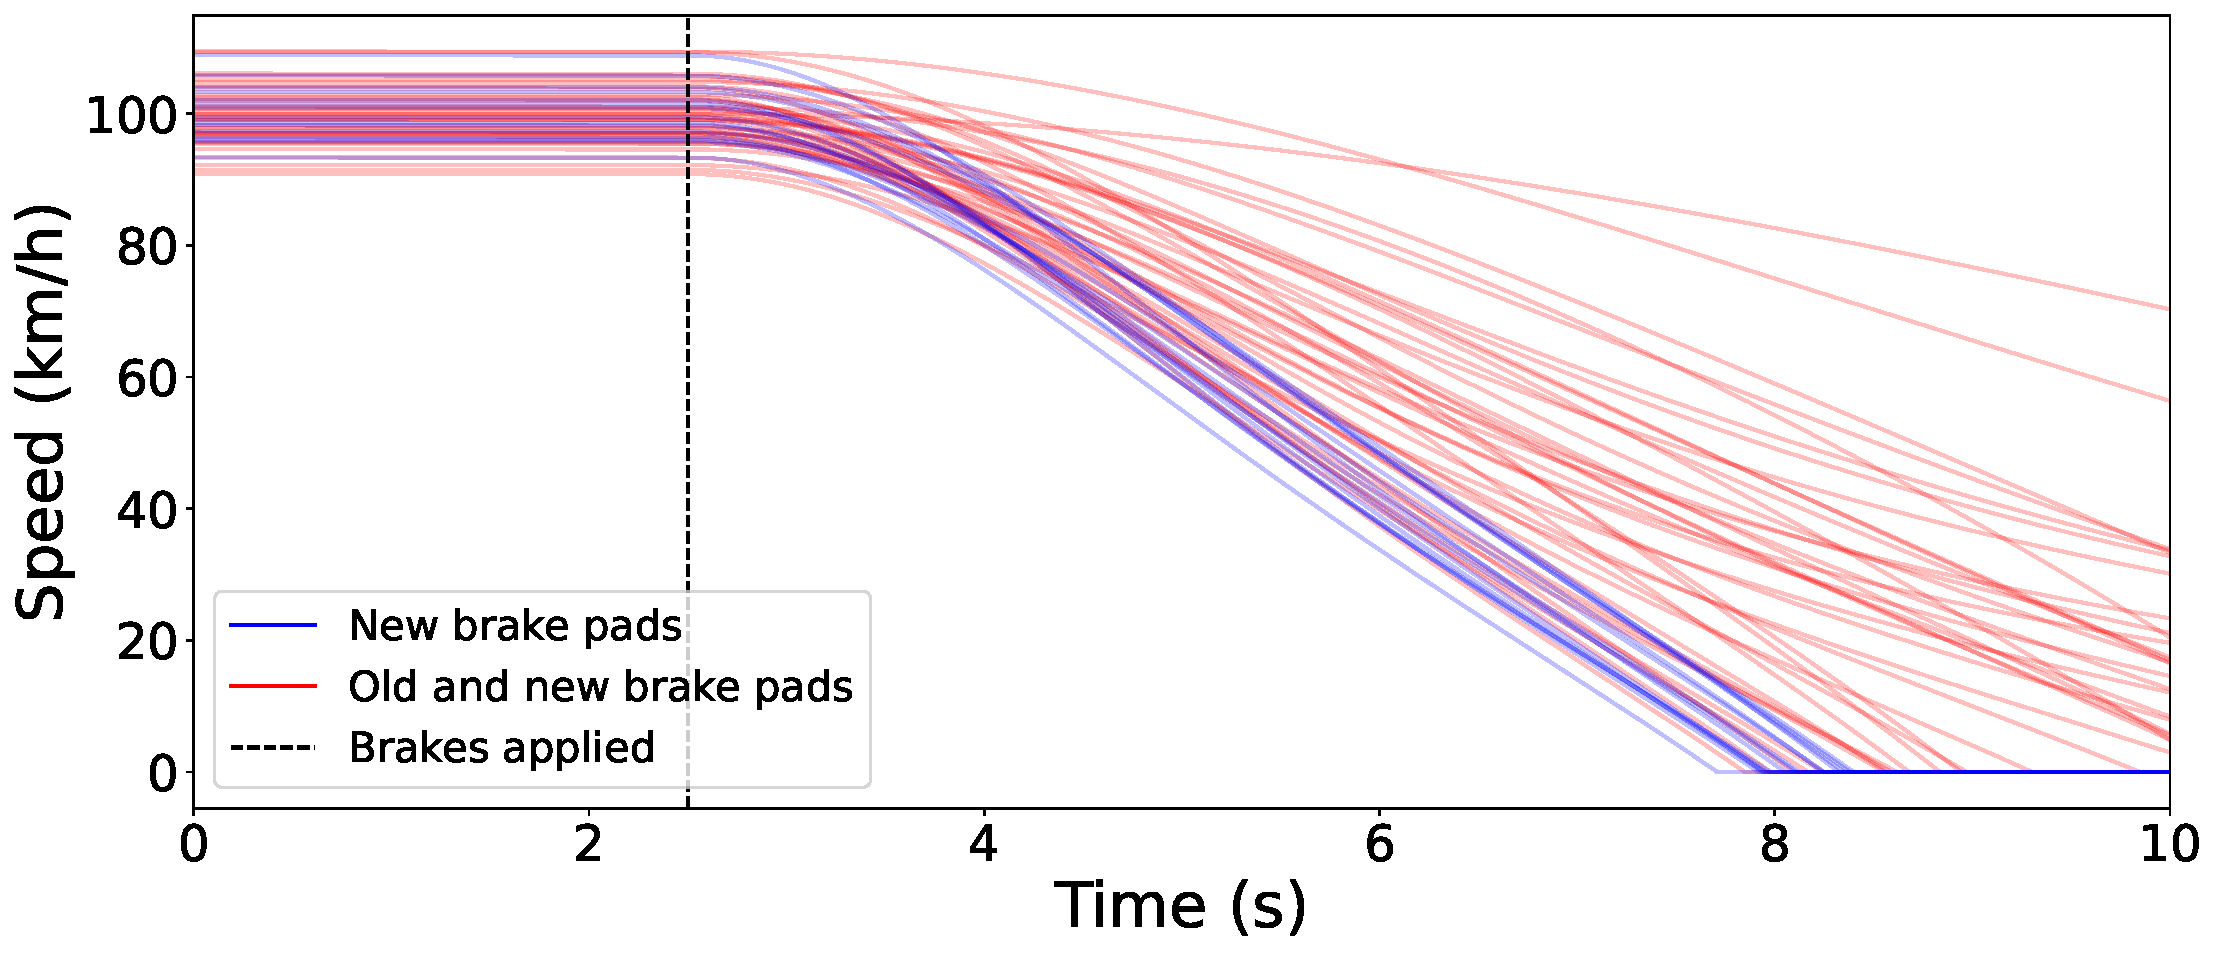
\includegraphics[height=5cm]{figures/causal/synthetic_example_newest2_nogray.pdf}
    %
    %
    %
    %

    \caption{The discrepancy between observational data and interventional behavior. The data only show the effect of aggressive braking on cars with new brake pads (blue). This differs from what \emph{would} be observed if aggressive braking were applied to the entire fleet of cars, encompassing both those with old and new brake pads (red).}
    
    %
    \label{fig:syn_ex}
\end{figure}

In the causal inference literature, any unmeasured quantity (e.g.\ brake pad age) that affects both some choice of action taken in the data (e.g.\ aggressive braking) and the resulting observation (e.g.\ speed) is referred to as an \emph{unmeasured confounder}.
In general, whenever an unmeasured confounder is present, a potential discrepancy arises between how the real-world process was observed to behave in the dataset and how it \emph{would} behave under certain interventions.
An obvious approach towards mitigating this possibility is to measure additional quantities that may affect the outcome of interest.
For example, if brake pad age were included in the data in the scenario above, then it would be possible to adjust for its effect on braking performance. 
However, in many cases, gathering additional data may be costly or impractical.
Moreover, even if this strategy is pursued, it is rarely possible to rule out the possibility of unmeasured confounding altogether, especially for complicated real-world problems \citep{tsiatis2019dynamic}. 
For example, in the scenario above, it is very conceivable that some other factor such as weather conditions could play a similar confounding role as brake pad age, and so would need also to be included in the data, and so on.
Analogous scenarios are also easily forthcoming for other application domains such as medicine and economics \citep{manski1995identification,tsiatis2019dynamic,hernan2020causal}.
%
As such, rather than attempting to sidestep the issue of unmeasured confounding, we instead propose a methodology for assessing twins using data that is robust to its presence. %

%
%
%
%
%


